\UseRawInputEncoding
\documentclass[a4paper,12pt]{article}

% ==============================================================================
% PACKAGES & HCMUS TEMPLATE FORMATTING
% ==============================================================================
\usepackage[utf8]{inputenc}
\usepackage[T1]{fontenc}
\usepackage{lmodern}
\usepackage{amsmath, amssymb, amsfonts, amsthm}
\usepackage{bm}
\usepackage{booktabs}
\usepackage{array}
\usepackage{multirow}
\usepackage{tabularx}
\usepackage{graphicx}
\usepackage{float}
\usepackage{caption}
\usepackage{subcaption}
\usepackage{xcolor}
\usepackage{enumitem}
\usepackage{hcmus-report-template}
\usepackage{tikz}
\usetikzlibrary{arrows.meta, positioning, shapes.geometric, calc, fit, backgrounds}

\setlength{\parskip}{0.35em}
\setlength{\parindent}{1.2em}
\renewcommand{\arraystretch}{1.15}

% Helper macro: includes experimental figure if already generated, otherwise renders a clean placeholder box
\newcommand{\IncludeExpFigure}[3]{%
    \IfFileExists{#1}{%
        \includegraphics[width=#2]{#1}%
    }{%
        \fbox{\parbox[c][3.2cm][c]{0.92\linewidth}{\centering \textbf{\small [Experimental Figure from Notebook]}\\[0.3em] {\scriptsize\nolinkurl{#1}}\\[0.3em] \footnotesize #3}}%
    }%
}

% ==============================================================================
% TITLE & METADATA (HCMUS SEMINAR REPORT TEMPLATE)
% ==============================================================================
\newcommand{\coursename}{CS420 — Introduction to Artificial Intelligence}
\newcommand{\reportname}{[S06] Diffusion Models: From Adding Noise to Generating Images}
\newcommand{\reporttitle}{SEMINAR REPORT}

\newcommand{\studentname}{Vong Chi Van (24125049)\\ Le Dat Phuc An (24125052)}

% Header
\lhead{\reporttitle}
\rhead{
University of Science - VNUHCM\\
\coursename
}

\begin{document}

\begin{titlepage}
\newcommand{\HRule}{\rule{\linewidth}{0.5mm}}
\centering

\textsc{\LARGE VNU-HCM}\\[0.5cm]
\textsc{\Large University of Science}\\[0.5cm]
\textsc{\large Faculty of Information Technology}\\[0.5cm]

\HRule \\[0.4cm]
{ 
\huge{\bfseries{\reporttitle}}\\[0.5cm]
\large{\bfseries{Topic: \reportname}}
}\\[0.4cm]
\HRule \\[0.5cm]

\textbf{\large Course: \coursename}\\[0.5cm]

\begin{minipage}[t]{0.55\textwidth}
\begin{flushleft} \large
\emph{Students:}\\
\studentname
\end{flushleft}
\end{minipage}
\\[0.6cm]
{\large \today}\\[0.6cm]


\includegraphics[scale=.20]{img/hcmus-logo.png}\\[0.5cm] 

\vfill
\end{titlepage}

\tableofcontents
\newpage

% ==============================================================================
% ABSTRACT
% ==============================================================================
\begin{abstract}
\noindent
Diffusion models have emerged as the foundational paradigm of modern Generative AI, surpassing Generative Adversarial Networks (GANs), Variational Autoencoders (VAEs), and Autoregressive Models in both visual sample fidelity and mode coverage. This report addresses the central guiding question: \textit{``How can learning to remove noise enable a model to generate brand-new images, and why does latent diffusion drastically reduce computational demands?''} Bridging probabilistic generative modeling with two landmark papers—\textbf{Denoising Diffusion Probabilistic Models (DDPM)} by Ho et al.\ (2020) \cite{ho2020denoising} and \textbf{Latent Diffusion Models (LDM)} by Rombach et al.\ (2022) \cite{rombach2022high}—we first contrast discriminative classifiers $P_\phi(Y\mid\mathbf{x})$ against generative models $p_\theta(\mathbf{x}, Y) = p_\theta(\mathbf{x}\mid Y)P(Y)$, demonstrating how learned class-conditional Gaussians $\mathcal{N}(\hat{\bm{\mu}}_c, \hat{\bm{\Sigma}}_c)$ function both as an optimal Bayes discriminator and as a data generator. We then present a comprehensive analysis of the forward Gaussian noising process $q(\mathbf{x}_t \mid \mathbf{x}_{t-1})$, variance-preserving $\beta_t$ scheduling across data resolutions, the closed-form jump $q(\mathbf{x}_t \mid \mathbf{x}_0)$, the reverse denoising chain $p_\theta(\mathbf{x}_{t-1} \mid \mathbf{x}_t)$, and the simplified noise-prediction objective $L_{\text{simple}}$. Crucially, we prove both intuitively and analytically (via bimodal posterior analysis and the Law of Total Variance) why re-injecting stochastic noise $+\sigma_t\mathbf{z}$ during reverse sampling is strictly necessary to break the symmetry of $L_2$ regression and prevent trajectories from collapsing onto a blurry dataset mean. We provide complete symbol specifications, a step-by-step 1D numerical worked example, an analysis of perceptual VAE compression combined with Cross-Attention conditioning in latent space, and controlled empirical experiments on 2D manifolds and MNIST ($28 \times 28$). Finally, we critically evaluate practical limitations regarding sequential sampling latency, prompt-based compositional control, training data copyright/memorization, and societal bias.
\end{abstract}

\vspace{0.5em}
\noindent\textbf{Keywords:} Generative AI, Denoising Diffusion Probabilistic Models (DDPM), Latent Diffusion Models (LDM), Variational Autoencoder (VAE), Cross-Attention, Bayes' Theorem.

\hrulefill

% ==============================================================================
% 1. INTRODUCTION
% ==============================================================================
\section{Introduction}

Synthesizing high-dimensional continuous signals such as natural images ($\mathbf{x} \in \mathbb{R}^{H \times W \times C}$) is a central challenge in artificial intelligence. Unlike supervised discriminative learning—which only seeks decision boundaries separating class labels—a generative model must capture the underlying probability distribution $p_{\text{data}}(\mathbf{x})$ of a complex, low-dimensional data manifold embedded in high-dimensional space, enabling the synthesis of novel samples $\mathbf{x}_{\text{new}} \sim p_\theta(\mathbf{x})$.

Prior to diffusion models, deep generative architectures faced the \textbf{Generative Learning Trilemma} \cite{xiao2022tackling}, struggling to simultaneously achieve \textit{(i) high sample sharpness}, \textit{(ii) full mode diversity}, and \textit{(iii) fast sampling}:
\begin{enumerate}[leftmargin=1.8em, itemsep=0.2em]
    \item \textbf{Variational Autoencoders (VAEs)} \cite{kingma2014auto} optimize a tractable Evidence Lower Bound (ELBO) and generate images in a single decoder forward pass, but suffer from \textbf{blurry samples} because a single-step Gaussian decoder averages over uncertain high-frequency details.
    \item \textbf{Generative Adversarial Networks (GANs)} \cite{goodfellow2014generative} achieve razor-sharp, single-step generation via an implicit minimax game ($\min_G \max_D$), but suffer from unstable saddle-point optimization and \textbf{mode collapse}—dropping minority modes of the data distribution.
    \item \textbf{Autoregressive Models (PixelRNN, PixelCNN)} \cite{oord2016pixel} factorize the exact log-likelihood $\prod_{i=1}^n p_\theta(x^{(i)} \mid x^{(<i)})$, achieving full mode coverage and sharp local contrast, but require $\mathcal{O}(n)$ sequential forward passes (one per pixel), making high-resolution synthesis prohibitively slow.
\end{enumerate}

\textbf{Guiding Question and Scope:} \textit{How can learning to remove noise enable a model to generate new images, and why does moving diffusion into a learned latent space resolve its computational bottleneck?}

The core insight of \textbf{Denoising Diffusion Probabilistic Models (DDPM)} \cite{sohl2015deep, ho2020denoising} is to decompose the difficult one-step mapping from standard Gaussian noise $\mathcal{N}(\mathbf{0}, \mathbf{I})$ to the data distribution $p_{\text{data}}(\mathbf{x}_0)$ into $T$ small, tractable steps ($T \approx 1000$). If a fixed forward process gradually corrupts a clean image $\mathbf{x}_0$ with small increments of Gaussian noise until $\mathbf{x}_T \sim \mathcal{N}(\mathbf{0}, \mathbf{I})$, then learning the reverse process—repeatedly predicting and subtracting small noise increments ($\mathbf{x}_T \to \mathbf{x}_{T-1} \to \dots \to \mathbf{x}_0$)—allows a neural network to start from pure random static and iteratively sculpt a realistic image. Furthermore, to overcome the immense computational cost of evaluating a full-resolution U-Net $1000$ times in pixel space, \textbf{Latent Diffusion Models (LDM)} \cite{rombach2022high} first compress images into the compact latent space of a pretrained Variational Autoencoder before running diffusion, reducing state dimensionality by $48\times$ and self-attention complexity by $4{,}096\times$.

% ==============================================================================
% 2. BACKGROUND & PAPER REVIEW
% ==============================================================================
\section{Background and Paper Review}

\subsection{Distinguishing Discriminative vs.\ Generative Models — Task 1}

Supervised classification and probabilistic modeling are fundamentally divided into \textbf{Discriminative} and \textbf{Generative} paradigms:

\begin{enumerate}[leftmargin=1.8em, itemsep=0.3em]
    \item \textbf{Pure Discriminative Models ($P_\phi(Y \mid \mathbf{x})$ — e.g., Logistic Regression, SVMs, MLP/ResNet Classifiers):}
    \begin{itemize}[leftmargin=1.4em, itemsep=0.15em]
        \item \textbf{What they learn:} Directly model the conditional probability $P_\phi(Y \mid \mathbf{x})$ or learn a separating hyperplane/decision boundary between classes to maximize classification accuracy, without modeling how the features $\mathbf{x}$ are distributed within each class.
        \item \textbf{Key Limitations:} Because a discriminative model only knows which side of a decision boundary a point $\mathbf{x}$ falls on, it \textbf{cannot generate new samples}. Furthermore, at out-of-distribution (OOD) coordinates far from the data manifold in empty space, a discriminative classifier remains \textbf{blindly overconfident ($\approx 100\%$)}, as the query still lies deep on one side of the separating hyperplane.
    \end{itemize}

    \item \textbf{Generative Models ($p_\theta(\mathbf{x}, Y) = p_\theta(\mathbf{x} \mid Y) P(Y)$ or $p_\theta(\mathbf{x})$ — e.g., Gaussian Bayes / GMM, VAEs, Diffusion Models):}
    \begin{itemize}[leftmargin=1.4em, itemsep=0.15em]
        \item \textbf{What they learn:} Explicitly model the underlying data distribution of each class. For instance, in a Gaussian generative model, the model estimates the empirical mean vector $\hat{\bm{\mu}}_c$ and covariance matrix $\hat{\bm{\Sigma}}_c$ for each class $c \in \{0, \dots, C-1\}$:
        \begin{equation}
            p_\theta(\mathbf{x} \mid Y = c) = \mathcal{N}\!\left(\mathbf{x};\, \hat{\bm{\mu}}_c, \hat{\bm{\Sigma}}_c\right) = \frac{1}{(2\pi)^{D/2}|\hat{\bm{\Sigma}}_c|^{1/2}} \exp\!\left(-\frac{1}{2}(\mathbf{x} - \hat{\bm{\mu}}_c)^\top \hat{\bm{\Sigma}}_c^{-1} (\mathbf{x} - \hat{\bm{\mu}}_c)\right)
        \end{equation}
        \item \textbf{Using a Learned Generative Model as a Discriminator via Bayes' Theorem:} Once the class distributions $p_\theta(\mathbf{x} \mid Y = c)$ and class priors $P(Y = c)$ are learned, the generative model directly acts as a \textbf{classifier (discriminator)} for any test point $\mathbf{x}_q$. It evaluates how likely $\mathbf{x}_q$ is under each class's learned Gaussian distribution and applies \textbf{Bayes' Rule}:
        \begin{equation}
        \begin{aligned}
            P_\theta(Y = c \mid \mathbf{x}_q) &= \frac{p_\theta(\mathbf{x}_q \mid Y = c)\, P(Y = c)}{\sum_{k=0}^{C-1} p_\theta(\mathbf{x}_q \mid Y = k)\, P(Y = k)}, \\
            \hat{y}_{\text{Bayes}}(\mathbf{x}_q) &= \arg\max_{c}\; p_\theta(\mathbf{x}_q \mid Y = c)\, P(Y = c)
        \end{aligned}
        \label{eq:bayes_classifier}
        \end{equation}
        The induced \textbf{Bayes decision boundary} between classes $c$ and $k$ is the locus of points where their weighted Gaussian likelihoods are equal: $p_\theta(\mathbf{x}\mid Y=c)P(Y=c) = p_\theta(\mathbf{x}\mid Y=k)P(Y=k)$.
        \item \textbf{Sampling \& Out-of-Distribution Detection:} Beyond classification, the marginal data density $p_\theta(\mathbf{x}) = \sum_{c} P(Y=c)\,p_\theta(\mathbf{x}\mid Y=c)$ enables the model to \textbf{detect out-of-distribution anomalies} (where $p_\theta(\mathbf{x}_{\text{OOD}}) \approx 0$) and \textbf{synthesize brand-new data samples} $\mathbf{x}_{\text{new}} \sim p_\theta(\mathbf{x})$.
    \end{itemize}
\end{enumerate}

\begin{table}[H]
\centering
\caption{Qualitative comparison of major generative model families (Task 1 — The Generative Learning Trilemma).}
\label{tab:task1_paradigms}
\footnotesize
\begin{tabularx}{\textwidth}{>{\raggedright\arraybackslash}p{2.4cm} >{\raggedright\arraybackslash}p{2.2cm} X >{\raggedright\arraybackslash}p{2.1cm} >{\raggedright\arraybackslash}p{2.1cm} >{\raggedright\arraybackslash}p{2.2cm}}
\toprule
\textbf{Model Family} & \textbf{Density $p_\theta(\mathbf{x})$} & \textbf{Training Mechanism \& Latent Structure} & \textbf{Sample Quality} & \textbf{Mode Coverage} & \textbf{Sampling Speed} \\
\midrule
\textbf{Autoregressive} \cite{oord2016pixel} (PixelRNN, PixelCNN) & Explicit, Exact (\textit{Exact MLE}) & Chain rule $\prod_{i=1}^n p_\theta(x^{(i)} \mid x^{(<i)})$ via causal masked convolutions; no global latent $\mathbf{z}$. & Sharp local contrast & Full (No mode collapse) & \textbf{Extremely Slow} ($\mathcal{O}(n)$ sequential pixel passes) \\
\addlinespace[0.3em]
\textbf{VAE} \cite{kingma2014auto} (Variational AE) & Explicit, Approx.\ (ELBO Bound) & Encoder $q_\phi(\mathbf{z}\mid\mathbf{x})$ + Decoder $p_\theta(\mathbf{x}\mid\mathbf{z})$ with $\dim(\mathbf{z}) \ll \dim(\mathbf{x})$; Reparameterization Trick. & \textbf{Blurry} (1-step $L_2$/BCE mode averaging) & Full, smooth latent manifold & \textbf{Very Fast} ($1$ Decoder forward pass) \\
\addlinespace[0.3em]
\textbf{GAN} \cite{goodfellow2014generative} (DCGAN, StyleGAN) & Implicit (Likelihood-free) & Adversarial minimax game $\min_G \max_D$ between Generator $G_\theta(\mathbf{z})$ and Discriminator $D_\phi(\mathbf{x})$. & \textbf{Razor Sharp} (\textit{Mode-seeking}) & \textbf{Poor} (Prone to \textit{Mode Collapse} \& instability) & \textbf{Very Fast} ($1$ Generator forward pass) \\
\addlinespace[0.3em]
\textbf{Pixel Diffusion} \cite{ho2020denoising} (DDPM) & Explicit, Approx.\ ($T$-step ELBO) & Fixed $T$-step Markov chain with $\dim(\mathbf{x}_t) = \dim(\mathbf{x}_0)$; U-Net predicts noise $\bm{\epsilon}_\theta(\mathbf{x}_t, t)$. & \textbf{SOTA Sharpness} & \textbf{Full} \& stable regression training & \textbf{Slow} ($T \approx 1000$ full-res U-Net passes) \\
\addlinespace[0.3em]
\textbf{Latent Diffusion} \cite{rombach2022high} (LDM / Stable Diff.) & Two-Stage ELBO (VAE + Diffusion) & Compresses $\mathbf{x}_0 \to \mathbf{z}_0$ via frozen Conv-VAE, then runs Cross-Attention U-Net on $\mathbf{z}_t$. & \textbf{SOTA} at high resolution & \textbf{Full} \& flexible multimodal control & \textbf{Fast / Practical} (Runs on $48\times$ smaller $\mathbf{z}_t$) \\
\bottomrule
\end{tabularx}
\end{table}

\subsection{Synthesis of Core Research Papers}

\begin{enumerate}[leftmargin=1.8em, itemsep=0.3em]
    \item \textbf{Required Paper — Ho, Jain \& Abbeel (NeurIPS 2020): \textit{``Denoising Diffusion Probabilistic Models'' (DDPM)} \cite{ho2020denoising}:}
    Building upon nonequilibrium thermodynamics \cite{sohl2015deep}, Ho et al.\ established a formal equivalence between hierarchical Markovian variational inference and denoising score matching with Langevin dynamics. Instead of training the reverse network to output the posterior mean image $\tilde{\bm{\mu}}_t$ directly, the authors reparameterized the U-Net as a \textbf{noise predictor $\bm{\epsilon}_\theta(\mathbf{x}_t, t)$} and discarded the theoretical variance-weighting coefficient in the ELBO to obtain $L_{\text{simple}}$. Empirically, Ho et al.\ demonstrated on CIFAR-10 ($32 \times 32$) that predicting $\bm{\epsilon}$ with $L_{\text{simple}}$ lowers the Fréchet Inception Distance (FID) from $13.51$ to $\mathbf{3.17}$—surpassing GANs while preserving full mode diversity.
    \item \textbf{Recommended Paper — Rombach et al.\ (CVPR 2022): \textit{``High-Resolution Image Synthesis With Latent Diffusion Models'' (LDM)} \cite{rombach2022high}:}
    Rombach et al.\ analyzed the rate-distortion trade-off of pixel-space DDPMs and observed that most model capacity and compute are wasted on imperceptible high-frequency pixel noise. They separated generation into: \textbf{(1) Perceptual Compression} via a convolutional autoencoder ($\mathcal{E}, \mathcal{D}$) that downsamples images by factor $f \in \{4, 8\}$ into a spatial latent grid $\mathbf{z}_0 = \mathcal{E}(\mathbf{x}_0)$, and \textbf{(2) Semantic Compression} via a diffusion model operating entirely in latent space $\mathbf{z}_t$, augmented with \textbf{Cross-Attention} layers for text, layout, and class conditioning.
\end{enumerate}

% ==============================================================================
% 3. METHOD & WORKED EXAMPLE
% ==============================================================================
\section{Method and Step-by-Step Worked Example}

\subsection{Forward Process, $\beta_t$ Schedule, Reverse Denoising, and Sampling — Task 2}

\subsubsection{The Forward Diffusion Process and Variance Preservation}
Given a clean data sample $\mathbf{x}_0 \sim q(\mathbf{x}_0)$, the \textbf{forward process} is a fixed Markov chain (\textbf{containing zero learnable parameters}) that gradually injects Gaussian noise over $T$ timesteps according to a variance schedule $\beta_1, \beta_2, \dots, \beta_T \in (0, 1)$:
\begin{equation}
    q(\mathbf{x}_{1:T} \mid \mathbf{x}_0) := \prod_{t=1}^T q(\mathbf{x}_t \mid \mathbf{x}_{t-1}), \qquad q(\mathbf{x}_t \mid \mathbf{x}_{t-1}) := \mathcal{N}\big(\mathbf{x}_t; \, \sqrt{1 - \beta_t}\,\mathbf{x}_{t-1}, \, \beta_t \mathbf{I}\big)
    \label{eq:forward_step}
\end{equation}
Via the \textit{Reparameterization Trick}, sampling $\mathbf{x}_t \sim q(\mathbf{x}_t \mid \mathbf{x}_{t-1})$ is expressed as:
\begin{equation}
    \mathbf{x}_t = \sqrt{1 - \beta_t}\,\mathbf{x}_{t-1} + \sqrt{\beta_t}\,\bm{\epsilon}_t, \qquad \bm{\epsilon}_t \sim \mathcal{N}(\mathbf{0}, \mathbf{I})
\end{equation}
\textbf{Why scale $\mathbf{x}_{t-1}$ by $\sqrt{1 - \beta_t}$?} Suppose $\text{Var}(\mathbf{x}_{t-1}) = \mathbf{I}$. Because $\mathbf{x}_{t-1}$ and $\bm{\epsilon}_t$ are independent, the variance of $\mathbf{x}_t$ is:
\begin{equation}
    \text{Var}(\mathbf{x}_t) = \left(\sqrt{1 - \beta_t}\right)^2 \text{Var}(\mathbf{x}_{t-1}) + \left(\sqrt{\beta_t}\right)^2 \text{Var}(\bm{\epsilon}_t) = (1 - \beta_t)\mathbf{I} + \beta_t\mathbf{I} = \mathbf{I}
\end{equation}
Because the squared coefficients sum to unity ($(1-\beta_t) + \beta_t = 1$), the forward chain is \textbf{Variance-Preserving (VP)}, ensuring $\mathbf{x}_T$ converges cleanly to $\mathcal{N}(\mathbf{0}, \mathbf{I})$ without exploding variance.

\subsubsection{Closed-Form $t$-Step Jump Property}
Defining $\alpha_t := 1 - \beta_t$ and $\bar{\alpha}_t := \prod_{s=1}^t \alpha_s$, and using the additivity of independent Gaussian variances, unrolling the recursion from $\mathbf{x}_0$ to $\mathbf{x}_t$ yields the exact marginal distribution at \textbf{any arbitrary timestep $t$ in $\mathcal{O}(1)$ operations}:
\begin{equation}
    q(\mathbf{x}_t \mid \mathbf{x}_0) = \mathcal{N}\big(\mathbf{x}_t; \, \sqrt{\bar{\alpha}_t}\,\mathbf{x}_0, \, (1 - \bar{\alpha}_t)\mathbf{I}\big) \quad \Longleftrightarrow \quad \mathbf{x}_t = \sqrt{\bar{\alpha}_t}\,\mathbf{x}_0 + \sqrt{1 - \bar{\alpha}_t}\,\bm{\epsilon}, \quad \bm{\epsilon} \sim \mathcal{N}(\mathbf{0}, \mathbf{I})
    \label{eq:closed_form_jump}
\end{equation}

\subsubsection{Purpose of the $\beta_t$ Schedule and Schedule Selection Across Data Domains}
If our sole objective in the forward process were to destroy $\mathbf{x}_0$ into $\mathcal{N}(\mathbf{0}, \mathbf{I})$, we could do so in a single step with $\beta_1 = 1$. \textbf{The forward $\beta_t$ schedule exists entirely to lay down ``stepping stones'' that make the reverse process $q(\mathbf{x}_{t-1} \mid \mathbf{x}_t)$ approximately Gaussian and learnable} (by Feller's Theorem, 1949):
\begin{itemize}[leftmargin=1.6em, itemsep=0.2em]
    \item \textbf{Why $\beta_1$ is tiny ($10^{-4}$) while $\beta_T$ is $200\times$ larger ($0.02$):} Near $t=1$, the clean image manifold $q(\mathbf{x}_0)$ is razor-sharp and highly non-Gaussian; a large step would mix multiple distinct modes, making $q(\mathbf{x}_0 \mid \mathbf{x}_1)$ multi-modal. Thus $\beta_1$ must be tiny. Near $t=T$, $q(\mathbf{x}_t)$ is already a smooth Gaussian bell curve, allowing much larger steps ($\beta_T = 0.02$).
    \item \textbf{Which $\beta_t$ schedule to choose for which data:}
    \begin{enumerate}[leftmargin=1.4em, itemsep=0.15em]
        \item \textit{Linear Schedule (Ho et al., 2020 \cite{ho2020denoising}, $\beta_1=10^{-4} \to \beta_{1000}=0.02$):} Designed for medium-resolution pixel images ($64^2$–$256^2$).
        \item \textit{Cosine Schedule (Nichol \& Dhariwal, 2021 \cite{nichol2021improved}):} Defines $\bar{\alpha}_t \propto \cos^2\big(\frac{t/T + s}{1+s}\frac{\pi}{2}\big)$. \textbf{Optimal for low-resolution images ($28\times 28$ MNIST, $32\times 32$ CIFAR-10)} and low-dimensional data, which lack spatial pixel redundancy and get destroyed too early under a linear schedule.
        \item \textit{Scaled-Linear Schedule (Rombach et al., 2022 \cite{rombach2022high}, $\beta_1=0.00085 \to \beta_{1000}=0.012$ quadratic):} \textbf{Optimal for VAE latent tensors ($\mathbf{z}_0 \in \mathbb{R}^{64\times 64\times 4}$)} where local pixel redundancy has already been compressed out.
        \item \textit{Shifted High-Noise Schedule (Hoogeboom et al., 2023):} \textbf{Required for high-resolution images ($512^2, 1024^2+$)}, where $16\times 16$ pixel patches average out independent noise, requiring larger $\beta_t$ to erase global low-frequency structure.
    \end{enumerate}
\end{itemize}

\subsubsection{Reverse Denoising Process, Noise Predictor \texorpdfstring{$\bm{\epsilon}_\theta$}{epsilon\_theta}, and Why \texorpdfstring{$+\sigma_t\mathbf{z}$}{+sigma\_t z} Is Mandatory}
The reverse process starts at $p(\mathbf{x}_T) = \mathcal{N}(\mathbf{0}, \mathbf{I})$ and learns Gaussian transitions:
\begin{equation}
    p_\theta(\mathbf{x}_{0:T}) := p(\mathbf{x}_T) \prod_{t=1}^T p_\theta(\mathbf{x}_{t-1} \mid \mathbf{x}_t), \qquad p_\theta(\mathbf{x}_{t-1} \mid \mathbf{x}_t) := \mathcal{N}\big(\mathbf{x}_{t-1}; \, \bm{\mu}_\theta(\mathbf{x}_t, t), \, \sigma_t^2 \mathbf{I}\big)
\end{equation}
Conditioned on $\mathbf{x}_0$, the forward posterior $q(\mathbf{x}_{t-1} \mid \mathbf{x}_t, \mathbf{x}_0) = \mathcal{N}(\tilde{\bm{\mu}}_t(\mathbf{x}_t, \mathbf{x}_0), \tilde{\beta}_t \mathbf{I})$ is tractable by Bayes' rule:
\begin{equation}
    \tilde{\beta}_t = \frac{1 - \bar{\alpha}_{t-1}}{1 - \bar{\alpha}_t}\beta_t, \qquad \tilde{\bm{\mu}}_t(\mathbf{x}_t, \mathbf{x}_0) = \frac{1}{\sqrt{\alpha_t}}\left(\mathbf{x}_t - \frac{\beta_t}{\sqrt{1 - \bar{\alpha}_t}}\bm{\epsilon}\right)
\end{equation}
Parameterizing the U-Net as a \textbf{noise predictor $\bm{\epsilon}_\theta(\mathbf{x}_t, t)$} yields the reverse sampling update for $t = T, \dots, 1$:
\begin{equation}
    \mathbf{x}_{t-1} = \underbrace{\frac{1}{\sqrt{\alpha_t}}\left(\mathbf{x}_t - \frac{\beta_t}{\sqrt{1 - \bar{\alpha}_t}}\bm{\epsilon}_\theta(\mathbf{x}_t, t)\right)}_{\bm{\mu}_\theta(\mathbf{x}_t, t)} + \sigma_t \mathbf{z}, \qquad \mathbf{z} \sim \mathcal{N}(\mathbf{0}, \mathbf{I}) \text{ (for } t > 1\text{; } \mathbf{z} = \mathbf{0} \text{ at } t = 1\text{)}
    \label{eq:reverse_sampling}
\end{equation}

\paragraph{Mathematical Proof of Why Omitting $+\sigma_t\mathbf{z}$ Collapses Samples to the Average Image:}
Because $L_{\text{simple}}$ is an $L_2$ regression loss, the optimal noise predictor outputs the conditional expectation $\bm{\epsilon}_\theta^*(\mathbf{x}_t, t) = \mathbb{E}[\bm{\epsilon} \mid \mathbf{x}_t] = \frac{\mathbf{x}_t - \sqrt{\bar{\alpha}_t}\mathbb{E}[\mathbf{x}_0 \mid \mathbf{x}_t]}{\sqrt{1-\bar{\alpha}_t}}$, which implies:
\begin{equation}
    \bm{\mu}_\theta^*(\mathbf{x}_t, t) = \mathbb{E}[\mathbf{x}_{t-1} \mid \mathbf{x}_t] = \frac{\sqrt{\bar{\alpha}_{t-1}}\beta_t}{1 - \bar{\alpha}_t}\underbrace{\mathbb{E}[\mathbf{x}_0 \mid \mathbf{x}_t]}_{\text{Blurry Posterior Mean}} + \frac{\sqrt{\alpha_t}(1 - \bar{\alpha}_{t-1})}{1 - \bar{\alpha}_t}\mathbf{x}_t
\end{equation}
Consider a realistic non-Gaussian bimodal dataset with two sharp modes at $x_0 = -1$ (Mode A) and $x_0 = +1$ (Mode B), whose global mean is $\mathbb{E}[x_0] = 0$ (where zero real data exists). By Bayes' rule, the exact posterior expectation is $\mathbb{E}[x_0 \mid x_t] = \tanh\!\big(\frac{\sqrt{\bar{\alpha}_t}}{1-\bar{\alpha}_t}x_t\big)$.
\begin{enumerate}[leftmargin=1.8em, itemsep=0.15em]
    \item \textbf{Without $+\sigma_t z$ ($\sigma_t = 0$):} During early steps ($t \approx T$, where $\bar{\alpha}_t \approx 0$), the mode-splitting term $\tanh(\cdot) \approx 0$ because the Gaussian clouds of Mode A and Mode B completely overlap. Thus, $\bm{\mu}_\theta^*(x_t, t) \approx \sqrt{\alpha_t}\,x_t$ ($\sqrt{\alpha_t} < 1$), which \textbf{actively contracts every trajectory inward toward the blurry mean $x_t = 0$}! By the Law of Total Variance $\text{Var}(x_{t-1}) = \text{Var}(\bm{\mu}_\theta^*) + \sigma_t^2$, omitting $+\sigma_t z$ strips out $\sigma_t^2$ of variance at every step, trapping samples at $x_0 = 0$.
    \item \textbf{How $+\sigma_t z$ Moves Samples Away from the Mean Into Sharp Modes:} In Stage 1 (large $t$), $+\sigma_t z$ fights the inward pull and keeps $x_t$ scattered at $\mathcal{O}(1)$ distance away from $0$. In Stage 2 (medium/small $t$), the forward noise clouds around $-1$ and $+1$ shrink and separate. Because $+\sigma_t z$ moved our sample to, say, $x_{t-1} = +0.5$ (a region visited during training only by Mode B), the $L_2$ vector field at $x_{t-1} = +0.5$ flips outward: $\tanh\!\big(\frac{\sqrt{\bar{\alpha}_{t-1}}}{1-\bar{\alpha}_{t-1}}x_{t-1}\big) \to +1$, locking the trajectory onto Mode B ($+1$).
\end{enumerate}

% TIKZ DIAGRAM FOR TASK 2 (BIDIRECTIONAL FORWARD & REVERSE PROCESS)
\begin{figure}[htbp]
\centering
\resizebox{\textwidth}{!}{%
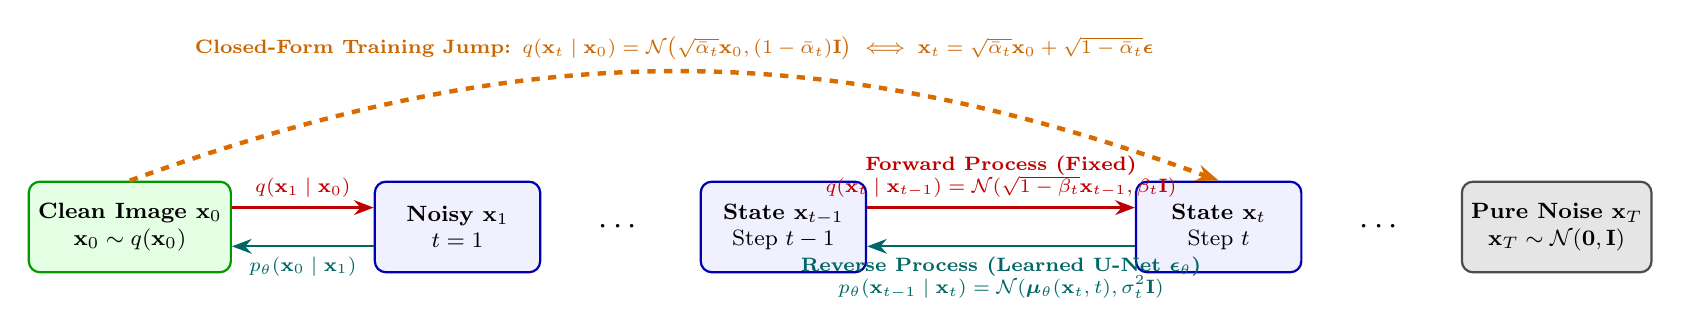
\begin{tikzpicture}[
    state/.style={rectangle, rounded corners=4pt, draw=blue!70!black, fill=blue!6, thick, minimum width=2.1cm, minimum height=1.15cm, align=center, font=\footnotesize},
    arrow_fwd/.style={-{Stealth[length=2.5mm]}, thick, draw=red!75!black},
    arrow_rev/.style={-{Stealth[length=2.5mm]}, thick, draw=teal!80!black},
    arrow_jump/.style={-{Stealth[length=2.8mm]}, ultra thick, dashed, draw=orange!85!black}
]
    \node[state, fill=green!10, draw=green!60!black] (x0) {\textbf{Clean Image $\mathbf{x}_0$}\\$\mathbf{x}_0 \sim q(\mathbf{x}_0)$};
    \node[state, right=1.8cm of x0] (x1) {\textbf{Noisy $\mathbf{x}_1$}\\$t = 1$};
    \node[right=0.6cm of x1, font=\bfseries\large] (dots1) {$\cdots$};
    \node[state, right=0.6cm of dots1] (xt1) {\textbf{State $\mathbf{x}_{t-1}$}\\Step $t-1$};
    \node[state, right=3.4cm of xt1] (xt) {\textbf{State $\mathbf{x}_t$}\\Step $t$};
    \node[right=0.6cm of xt, font=\bfseries\large] (dots2) {$\cdots$};
    \node[state, fill=gray!20, draw=gray!60!black, right=0.6cm of dots2] (xT) {\textbf{Pure Noise $\mathbf{x}_T$}\\$\mathbf{x}_T \sim \mathcal{N}(\mathbf{0}, \mathbf{I})$};

    % Forward arrows (Top)
    \draw[arrow_fwd] ([yshift=7pt]x0.east) -- node[above, font=\scriptsize, text=red!75!black] {$q(\mathbf{x}_1\mid\mathbf{x}_0)$} ([yshift=7pt]x1.west);
    \draw[arrow_fwd] ([yshift=7pt]xt1.east) -- node[above, font=\scriptsize, align=center, text=red!75!black] {\textbf{Forward Process (Fixed)}\\$q(\mathbf{x}_t\mid\mathbf{x}_{t-1}) = \mathcal{N}(\sqrt{1-\beta_t}\mathbf{x}_{t-1}, \beta_t\mathbf{I})$} ([yshift=7pt]xt.west);

    % Reverse arrows (Bottom)
    \draw[arrow_rev] ([yshift=-7pt]x1.west) -- node[below, font=\scriptsize, text=teal!80!black] {$p_\theta(\mathbf{x}_0\mid\mathbf{x}_1)$} ([yshift=-7pt]x0.east);
    \draw[arrow_rev] ([yshift=-7pt]xt.west) -- node[below, font=\scriptsize, align=center, text=teal!80!black] {\textbf{Reverse Process (Learned U-Net $\bm{\epsilon}_\theta$)}\\$p_\theta(\mathbf{x}_{t-1}\mid\mathbf{x}_t) = \mathcal{N}(\bm{\mu}_\theta(\mathbf{x}_t, t), \sigma_t^2\mathbf{I})$} ([yshift=-7pt]xt1.east);

    % Closed-form jump (Curved top)
    \draw[arrow_jump] (x0.north) to[out=20, in=160] node[above, font=\scriptsize\bfseries, text=orange!80!black] {Closed-Form Training Jump: $q(\mathbf{x}_t \mid \mathbf{x}_0) = \mathcal{N}\big(\sqrt{\bar{\alpha}_t}\mathbf{x}_0, (1-\bar{\alpha}_t)\mathbf{I}\big) \iff \mathbf{x}_t = \sqrt{\bar{\alpha}_t}\mathbf{x}_0 + \sqrt{1-\bar{\alpha}_t}\bm{\epsilon}$} (xt.north);
\end{tikzpicture}%
}
\caption{Bidirectional diagram illustrating the forward Gaussian noising process (fixed schedule $\beta_t$) and the learned reverse denoising process (driven by U-Net noise predictor $\bm{\epsilon}_\theta(\mathbf{x}_t, t)$) in DDPM (Task 2).}
\label{fig:ddpm_bidirectional}
\end{figure}

% ==============================================================================
% 3.2 SECTION III & TASK 3: FORMAL EQUATIONS & 1D WORKED NUMERICAL EXAMPLE
% ==============================================================================
\subsection{Formal Equation Specifications and 1D Worked Numerical Example — Section III \& Task 3}

In accordance with Section III of the seminar specification, Table \ref{tab:eq_symbols} defines every symbol, unit/value range, and modeling assumption for the two required equations:
\begin{align}
    q(\mathbf{x}_t \mid \mathbf{x}_{t-1}) &= \mathcal{N}\big(\sqrt{1 - \beta_t}\,\mathbf{x}_{t-1}, \, \beta_t \mathbf{I}\big) \tag{Equation 1}\\
    L_{\text{simple}}(\theta) &= \mathbb{E}_{t, \mathbf{x}_0, \bm{\epsilon}}\Big[\big\|\bm{\epsilon} - \bm{\epsilon}_\theta(\mathbf{x}_t, t)\big\|^2\Big] \tag{Equation 2}
\end{align}

\begin{table}[H]
\centering
\caption{Complete symbol definitions, value ranges/units, and modeling assumptions for Section III.}
\label{tab:eq_symbols}
\footnotesize
\begin{tabularx}{\textwidth}{>{\raggedright\arraybackslash}p{1.9cm} >{\raggedright\arraybackslash}p{3.6cm} >{\raggedright\arraybackslash}p{4.2cm} X}
\toprule
\textbf{Symbol} & \textbf{Mathematical Definition} & \textbf{Units \& Value Range} & \textbf{Modeling Assumptions} \\
\midrule
$t$ & Discrete diffusion timestep index & Unitless integer: $t \in \{1, 2, \dots, T\}$ ($T=1000$) & Finite-horizon discrete-time Markov chain; sampled via $t \sim \text{Uniform}(\{1, \dots, T\})$ during training. \\
\addlinespace[0.25em]
$\mathbf{x}_0$ & Initial clean data sample (image tensor) & Normalized dimensionless pixel intensity: $\mathbf{x}_0 \in [-1, 1]^D$ ($D = H\cdot W\cdot C$) & Continuous state linearly rescaled from $[0, 255]$ integers to $[-1, 1]$ to match the zero-mean, unit-variance prior $\mathcal{N}(\mathbf{0}, \mathbf{I})$. \\
\addlinespace[0.25em]
$\mathbf{x}_{t-1}, \mathbf{x}_t$ & Noisy latent states at steps $t-1$ and $t$ & Continuous real tensors: $\mathbf{x}_{t-1}, \mathbf{x}_t \in \mathbb{R}^D$ & \textbf{Dimension-preserving latent space:} Every latent $\mathbf{x}_t$ has the exact same dimensionality $D$ as $\mathbf{x}_0$. \\
\addlinespace[0.25em]
$q(\mathbf{x}_t \mid \mathbf{x}_{t-1})$ & Forward Markov transition probability density & Probability density: $q \ge 0$, $\int q(\mathbf{x}_t\mid\mathbf{x}_{t-1})d\mathbf{x}_t = 1$ & \textbf{Markov Property:} $q(\mathbf{x}_t \mid \mathbf{x}_{0:t-1}) = q(\mathbf{x}_t \mid \mathbf{x}_{t-1})$ (memoryless conditioned on $\mathbf{x}_{t-1}$). \\
\addlinespace[0.25em]
$\beta_t$ & Forward noise variance schedule at step $t$ & Unitless variance fraction: $\beta_t \in (0, 1)$, typically $10^{-4} \le \beta_t \le 0.02$ & Fixed hyperparameter schedule ($\beta_1 < \dots < \beta_T$) chosen small enough ($\beta_t \ll 1$) that reverse transitions are Gaussian. \\
\addlinespace[0.25em]
$\sqrt{1 - \beta_t}$ & Signal attenuation (contraction) factor & Unitless scalar: $\sqrt{1-\beta_t} \in (0, 1)$ & Variance-preserving scaling: $(\sqrt{1-\beta_t})^2 + (\sqrt{\beta_t})^2 = 1$. \\
\addlinespace[0.25em]
$\mathbf{I}$ & $D \times D$ Identity covariance matrix & Dimensionless matrix $\mathbf{I} \in \{0, 1\}^{D\times D}$ & \textbf{Isotropic Gaussian assumption:} Noise is independent and identically distributed (i.i.d.) across all pixels/channels. \\
\addlinespace[0.25em]
$L_{\text{simple}}$ & Simplified unweighted noise MSE objective & Non-negative real scalar: $L_{\text{simple}} \in [0, \infty)$ & Drops the ELBO weight $\frac{\beta_t^2}{2\sigma_t^2\alpha_t(1-\bar{\alpha}_t)}$ to upweight harder, high-noise semantic steps ($t \gg 1$). \\
\addlinespace[0.25em]
$\mathbb{E}_{t, \mathbf{x}_0, \bm{\epsilon}}[\cdot]$ & Joint expectation over $(t, \mathbf{x}_0, \bm{\epsilon})$ & Approximated via mini-batch average of size $B$ & Assumes $t$, $\mathbf{x}_0 \sim q(\mathbf{x}_0)$, and $\bm{\epsilon} \sim \mathcal{N}(\mathbf{0}, \mathbf{I})$ are drawn independently. \\
\addlinespace[0.25em]
$\bm{\epsilon}$ & Ground-truth standard normal noise realization & Continuous real tensor: $\bm{\epsilon} \in \mathbb{R}^D$, $\bm{\epsilon} \sim \mathcal{N}(\mathbf{0}, \mathbf{I})$ & Zero mean, unit variance ($\approx 99.7\%$ of values in $[-3, +3]$). \\
\addlinespace[0.25em]
$\bm{\epsilon}_\theta(\mathbf{x}_t, t)$ & Neural network (U-Net) noise predictor & Continuous real tensor: $\bm{\epsilon}_\theta(\mathbf{x}_t, t) \in \mathbb{R}^D$ & Shares weights $\theta$ across all $T$ steps via sinusoidal timestep embeddings. \\
\bottomrule
\end{tabularx}
\end{table}

\subsubsection{Step-by-Step 1D Worked Numerical Example (Task 3)}
Consider a 1-dimensional forward noising step ($D = 1$, representing a single normalized pixel) at $t = 1$:
\begin{enumerate}[leftmargin=1.8em, itemsep=0.25em]
    \item \textbf{Chosen Input Values:}
    \begin{itemize}[leftmargin=1.4em, itemsep=0.1em]
        \item Clean normalized pixel intensity: $\mathbf{x_0 = 0.80}$ (in $[-1, 1]$, corresponding to $229.5 \approx 230$ in 8-bit grayscale).
        \item Variance schedule at step $t = 1$: $\mathbf{\beta_1 = 0.19}$ (chosen so $1 - \beta_1 = 0.81$ has an exact rational square root $\sqrt{0.81} = 0.90$; representative of a 5-step illustrative schedule).
        \item Realized standard normal noise sample drawn from $\epsilon \sim \mathcal{N}(0, 1)$: $\mathbf{\epsilon = -0.50}$.
    \end{itemize}
    \item \textbf{Step 1 — Compute Parameters of the Forward Distribution $q(x_1 \mid x_0 = 0.80)$:}
    \begin{itemize}[leftmargin=1.4em, itemsep=0.1em]
        \item Signal retention factor: $\alpha_1 = 1 - \beta_1 = 1 - 0.19 = 0.81 \implies \sqrt{1 - \beta_1} = \sqrt{0.81} = \mathbf{0.90}$.
        \item \textbf{Stochastic Expectation (Conditional Mean):}
        \begin{equation}
            \mu_1 = \mathbb{E}[x_1 \mid x_0 = 0.80] = \sqrt{1 - \beta_1}\, x_0 = 0.90 \times 0.80 = \mathbf{0.7200}
        \end{equation}
        \item \textbf{Conditional Variance and Standard Deviation:}
        \begin{equation}
            \sigma_1^2 = \beta_1 = \mathbf{0.1900} \implies \sigma_1 = \sqrt{\beta_1} = \sqrt{0.19} \approx \mathbf{0.4359}
        \end{equation}
        Hence, $q(x_1 \mid x_0 = 0.80) = \mathcal{N}(0.7200, \, 0.1900)$.
    \end{itemize}
    \item \textbf{Step 2 — Calculate the Realized Noisy Pixel $x_1$ for $\epsilon = -0.50$:}
    \begin{equation}
        x_1 = \sqrt{1 - \beta_1}\, x_0 + \sqrt{\beta_1}\, \epsilon = 0.7200 + (0.4359 \times (-0.50)) = 0.7200 - 0.21795 = \mathbf{0.5021}
    \end{equation}
    \item \textbf{Step 3 — Physical Interpretation of the Stochastic Expectation $\mathbb{E}[x_1 \mid x_0] = 0.7200$:}
    Since $\mathbb{E}[\epsilon] = 0$, averaging over infinitely many random realizations of $\epsilon \sim \mathcal{N}(0, 1)$ yields:
    \begin{equation}
        \mathbb{E}_{\epsilon \sim \mathcal{N}(0,1)}[x_1 \mid x_0] = \sqrt{1 - \beta_1}\,x_0 + \sqrt{\beta_1}\underbrace{\mathbb{E}[\epsilon]}_{=0} = 0.90\,x_0 = 0.7200 < x_0
    \end{equation}
    \textit{Interpretation:} Even when random noise fluctuations average out, the forward diffusion step \textbf{systematically contracts the expected signal amplitude toward $0$} by factor $\sqrt{1-\beta_t} = 0.90$. Over $T$ steps, $\mathbb{E}[x_T \mid x_0] = \sqrt{\bar{\alpha}_T}\,x_0 \to 0$, erasing each image's initial mean so all inputs merge into the zero-mean prior $\mathcal{N}(0, 1)$.
    \item \textbf{Step 4 — Worked Calculation of $L_{\text{simple}}$ and Reverse Denoising ($x_1 \to \hat{x}_0$):}
    Suppose the neural network receives $(x_1 = 0.5021, \, t = 1)$ and outputs predicted noise $\epsilon_\theta(0.5021, 1) = \mathbf{-0.30}$.
    \begin{itemize}[leftmargin=1.4em, itemsep=0.1em]
        \item \textbf{Sample Loss $L_{\text{simple}}$:}
        \begin{equation}
            \ell_{\text{simple}} = \big\|\epsilon - \epsilon_\theta(x_1, 1)\big\|^2 = (-0.50 - (-0.30))^2 = (-0.20)^2 = \mathbf{0.0400}
        \end{equation}
        \item \textbf{Reverse Denoising Step (\ref{eq:reverse_sampling}) at $t=1$ (with $z=0, \, \alpha_1 = \bar{\alpha}_1 = 0.81$):}
        \begin{equation}
            \hat{x}_0 = \frac{1}{\sqrt{\alpha_1}}\left(x_1 - \frac{\beta_1}{\sqrt{1 - \bar{\alpha}_1}}\epsilon_\theta(x_1, 1)\right) = \frac{1}{0.90}\big(0.5021 - 0.4359 \times (-0.30)\big) = \frac{0.6329}{0.90} \approx \mathbf{0.7032}
        \end{equation}
        Once trained to optimality ($\epsilon_\theta = \epsilon = -0.50$), we recover $\hat{x}_0 = \frac{0.5021 - 0.4359(-0.50)}{0.90} = \frac{0.7200}{0.90} = \mathbf{0.8000 = x_0}$.
    \end{itemize}
\end{enumerate}

% ==============================================================================
% 3.3 TASK 5: LATENT DIFFUSION MODELS (VAE + LATENT SPACE + CROSS-ATTENTION)
% ==============================================================================
\subsection{Latent Diffusion Models (LDMs): Perceptual VAE Compression \& Cross-Attention — Task 5}

\subsubsection{Perceptual Compression via Frozen Autoencoder ($\mathcal{E}, \mathcal{D}$) and Latent Space Operations}
In pixel-space DDPMs, $\mathbf{x}_t$ retains the full resolution of $\mathbf{x}_0$ (e.g., $512 \times 512 \times 3 = 786{,}432$ dimensions), making 1000 U-Net evaluations computationally prohibitive. Rombach et al.\ (2022) \cite{rombach2022high} overcome this via a two-stage pipeline (Figure \ref{fig:ldm_pipeline}):
\begin{enumerate}[leftmargin=1.8em, itemsep=0.2em]
    \item \textbf{Perceptual Convolutional VAE ($\mathcal{E}, \mathcal{D}$):} A Fully Convolutional VAE is pretrained with a perceptual loss (LPIPS), a patch-based adversarial discriminator, and a light KL penalty (\textit{KL-reg}) to map $\mathbf{x}_0 \in \mathbb{R}^{H \times W \times 3}$ into a 3D spatial latent tensor $\mathbf{z}_0 = \mathcal{E}(\mathbf{x}_0) \in \mathbb{R}^{h \times w \times c}$ downsampled by factor $f = H/h = W/w = 2^m$.
    \begin{itemize}[leftmargin=1.4em, itemsep=0.1em]
        \item In Stable Diffusion ($f = 8, c = 4$), a $512 \times 512 \times 3$ image ($786{,}432$ scalars) is compressed into $\mathbf{z}_0 \in \mathbb{R}^{64 \times 64 \times 4}$ ($16{,}384$ scalars)—a \textbf{$48\times$ reduction in tensor size}!
        \item Because 2D self-attention scales quadratically with spatial area $\mathcal{O}((H\cdot W)^2)$, reducing spatial dimensions by $f=8$ reduces token count by $f^2 = 64\times$ and \textbf{cuts self-attention memory and FLOPs by $f^4 = 8^4 = 4{,}096\times$}!
    \end{itemize}
    \item \textbf{Diffusion in Latent Space ($\mathbf{z}_0 \leftrightarrow \mathbf{z}_T$):} With $\mathcal{E}$ and $\mathcal{D}$ frozen, forward noising $\mathbf{z}_t = \sqrt{\bar{\alpha}_t}\mathbf{z}_0 + \sqrt{1-\bar{\alpha}_t}\bm{\epsilon}$ and reverse U-Net denoising $\bm{\epsilon}_\theta(\mathbf{z}_t, t)$ run entirely on $\mathbf{z}_t \in \mathbb{R}^{64 \times 64 \times 4}$. At the end of the $T$-step reverse loop, a \textbf{single forward pass} through the frozen decoder $\hat{\mathbf{x}}_0 = \mathcal{D}(\hat{\mathbf{z}}_0)$ reconstructs the full $512 \times 512 \times 3$ RGB image.
\end{enumerate}

\subsubsection{Multimodal Conditioning via Cross-Attention}
To condition generation on text prompts or semantic maps $y$, a domain encoder $\tau_\theta(y) \in \mathbb{R}^{M \times d_\tau}$ (e.g., a pretrained CLIP text transformer) projects $y$ into $M$ token embeddings, which are injected into intermediate U-Net layers via \textbf{Multi-Head Cross-Attention}:
\begin{equation}
    \text{Attention}(\mathbf{Q}, \mathbf{K}, \mathbf{V}) = \text{softmax}\!\left(\frac{\mathbf{Q}\mathbf{K}^T}{\sqrt{d}}\right)\mathbf{V}, \quad
    \begin{cases}
        \mathbf{Q} = \varphi_i(\mathbf{z}_t)\,\mathbf{W}_Q^{(i)} & \text{(from spatial latent }\mathbf{z}_t\text{)}\\
        \mathbf{K} = \tau_\theta(y)\,\mathbf{W}_K^{(i)} & \text{(from prompt }y\text{)}\\
        \mathbf{V} = \tau_\theta(y)\,\mathbf{W}_V^{(i)} & \text{(from prompt }y\text{)}
    \end{cases}
\end{equation}
The conditioned Latent Diffusion training objective is:
\begin{equation}
    L_{\text{LDM}}(\theta) := \mathbb{E}_{\mathcal{E}(\mathbf{x}_0), \, y, \, \bm{\epsilon} \sim \mathcal{N}(\mathbf{0}, \mathbf{I}), \, t}\Big[\big\|\bm{\epsilon} - \bm{\epsilon}_\theta\big(\mathbf{z}_t, \, t, \, \tau_\theta(y)\big)\big\|^2\Big]
\end{equation}

% TIKZ DIAGRAM FOR TASK 5 (LATENT DIFFUSION PIPELINE)
\begin{figure}[htbp]
\centering
\resizebox{\textwidth}{!}{%
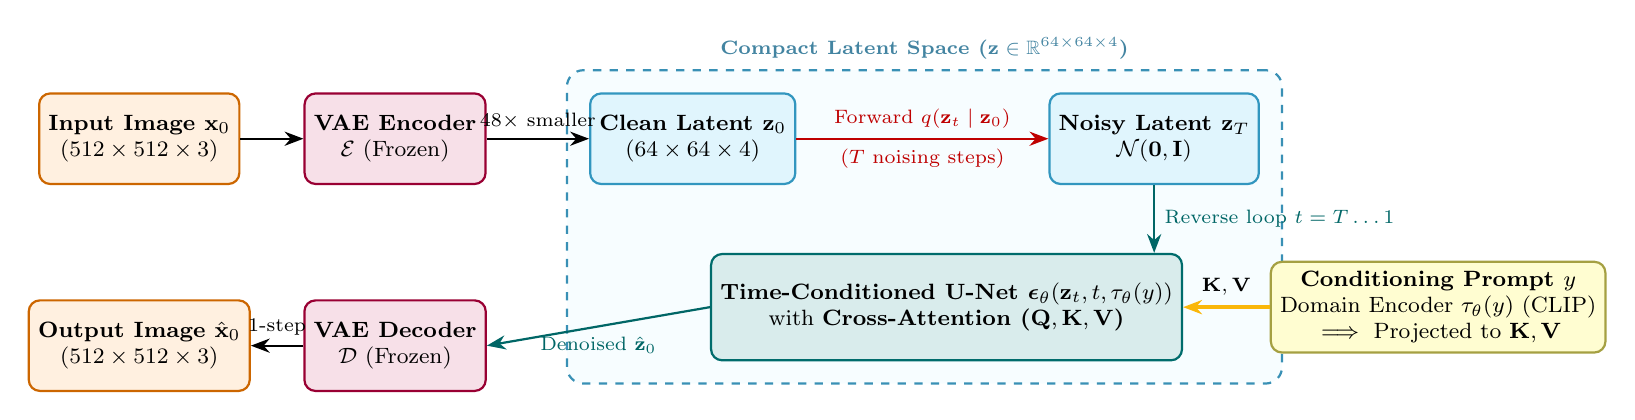
\begin{tikzpicture}[
    box/.style={rectangle, rounded corners=4pt, draw=black!75, thick, align=center, font=\footnotesize, minimum height=1.15cm},
    pixelbox/.style={box, fill=orange!12, draw=orange!80!black, minimum width=2.4cm},
    vaebox/.style={box, fill=purple!12, draw=purple!80!black, minimum width=2.0cm},
    latbox/.style={box, fill=cyan!12, draw=cyan!75!black, minimum width=2.5cm},
    unetbox/.style={box, fill=teal!15, draw=teal!85!black, minimum width=4.6cm, minimum height=1.35cm},
    condbox/.style={box, fill=yellow!18, draw=yellow!60!black, minimum width=3.1cm},
    arr/.style={-{Stealth[length=2.4mm]}, thick}
]
    % Top row: Input -> Encoder -> Clean Latent z0 -> Noisy Latent zT
    \node[pixelbox] (x0) {\textbf{Input Image $\mathbf{x}_0$}\\$(512\times 512\times 3)$};
    \node[vaebox, right=0.8cm of x0] (enc) {\textbf{VAE Encoder}\\$\mathcal{E}$ (Frozen)};
    \node[latbox, right=1.3cm of enc] (z0) {\textbf{Clean Latent $\mathbf{z}_0$}\\$(64\times 64\times 4)$};
    \node[latbox, right=3.2cm of z0] (zT) {\textbf{Noisy Latent $\mathbf{z}_T$}\\$\mathcal{N}(\mathbf{0}, \mathbf{I})$};

    % Bottom row: Output <- Decoder <- Denoised z0 <- Reverse U-Net <- Conditioning
    \node[pixelbox, below=1.45cm of x0] (xhat) {\textbf{Output Image $\hat{\mathbf{x}}_0$}\\$(512\times 512\times 3)$};
    \node[vaebox, below=1.45cm of enc] (dec) {\textbf{VAE Decoder}\\$\mathcal{D}$ (Frozen)};
    \node[unetbox, below=1.45cm of $(z0)!0.55!(zT)$] (unet) {\textbf{Time-Conditioned U-Net $\bm{\epsilon}_\theta(\mathbf{z}_t, t, \tau_\theta(y))$}\\with \textbf{Cross-Attention ($\mathbf{Q}, \mathbf{K}, \mathbf{V}$)}};
    \node[condbox, right=1.1cm of unet] (cond) {\textbf{Conditioning Prompt $y$}\\Domain Encoder $\tau_\theta(y)$ (CLIP)\\$\implies$ Projected to $\mathbf{K}, \mathbf{V}$};

    % Connections
    \draw[arr] (x0) -- (enc);
    \draw[arr] (enc) -- node[above, font=\scriptsize] {$48\times$ smaller} (z0);
    \draw[arr, draw=red!75!black] (z0) -- node[above, font=\scriptsize, text=red!75!black] {Forward $q(\mathbf{z}_t\mid\mathbf{z}_0)$} node[below, font=\scriptsize, text=red!75!black] {($T$ noising steps)} (zT);
    \draw[arr, draw=teal!80!black] (zT.south) -- node[right, font=\scriptsize, text=teal!80!black] {Reverse loop $t=T\dots 1$} (unet.north -| zT.south);
    \draw[arr, draw=teal!80!black] (unet.west) -- node[below, font=\scriptsize, text=teal!80!black] {Denoised $\hat{\mathbf{z}}_0$} (dec.east);
    \draw[arr] (dec) -- node[above, font=\scriptsize] {1-step} (xhat);
    \draw[arr, ultra thick, draw=yellow!45!orange] (cond.west) -- node[above, font=\scriptsize\bfseries] {$\mathbf{K}, \mathbf{V}$} (unet.east);

    % Background group box for Latent Space
    \begin{scope}[on background layer]
        \node[draw=cyan!70!black, dashed, thick, rounded corners=6pt, fill=cyan!3, inner sep=8pt, fit=(z0) (zT) (unet), label={[font=\scriptsize\bfseries, text=cyan!60!black]above:Compact Latent Space ($\mathbf{z} \in \mathbb{R}^{64\times 64\times 4}$)}] {};
    \end{scope}
\end{tikzpicture}%
}
\caption{Complete Latent Diffusion Model (LDM) pipeline: Perceptual compression via frozen VAE ($\mathcal{E}, \mathcal{D}$), diffusion operations in latent space $\mathbf{z}$, and Cross-Attention conditioning (Task 5, adapted from Rombach et al., 2022 \cite{rombach2022high}).}
\label{fig:ldm_pipeline}
\end{figure}

% ==============================================================================
% 4. RESULTS AND DISCUSSION
% ==============================================================================
\section{Results and Discussion}

In strict compliance with the seminar guidelines (distinguishing experiments developed by our team from findings reported in the research literature), we divide our results into two parts.

\subsection{Part A: Empirical Experiments Developed by Our Team (MNIST $28 \times 28$ \& 2D Manifolds)}
\label{sec:exp_task1}
We implemented a self-contained experimental suite in \nolinkurl{experiments/task1_generative_paradigms_comparison.ipynb}, executed on an NVIDIA GeForce RTX 5060 Ti GPU (PyTorch 2.10, CUDA 12.8):

\begin{enumerate}[leftmargin=1.8em, itemsep=0.25em]
    \item \textbf{Experiment 1A — Discriminative Classifier vs.\ Generative Model Used as a Discriminator (Bayes' Rule) \& Generator (Figure \ref{fig:exp_disc_gen}):}
    \begin{itemize}[leftmargin=1.4em, itemsep=0.15em]
        \item \textbf{Pure Discriminative Classifier $P_\phi(Y\mid\mathbf{x})$ (Figure \ref{fig:exp_disc_gen}a):} On our 4-class 2D tilted-Gaussian benchmark, the MLP classifier achieves $\mathbf{100.0\%}$ test accuracy by partitioning the plane into four quadrants. However, because it only models decision boundaries, it outputs $\mathbf{100.0\%}$ confidence at the out-of-distribution point $\mathbf{x}_{\text{OOD}} = (4.5, 4.5)$ in empty space and cannot generate new samples.
        \item \textbf{Generative Model Used as a Discriminator via Bayes' Rule (Figure \ref{fig:exp_disc_gen}b):} The generative model first fits a 2D Gaussian $\mathcal{N}(\hat{\bm{\mu}}_c, \hat{\bm{\Sigma}}_c)$ to each class $c \in \{0, 1, 2, 3\}$ (visualized by the $1\sigma, 2\sigma, 3\sigma$ covariance ellipses). Using \textbf{Bayes' Theorem}, $P_\theta(Y=c\mid\mathbf{x}) \propto p_\theta(\mathbf{x}\mid Y=c)P(Y=c)$, it induces exact \textbf{Bayes Decision Boundaries} where adjacent Gaussian likelihoods balance, achieving $\mathbf{100.0\%}$ test classification accuracy. For the query point $\mathbf{x}_q = (-1.15, 1.25)$ (yellow star), it compares class likelihoods $p_\theta(\mathbf{x}_q\mid Y=1) = 4.41 \times 10^{-2}$ vs.\ $p_\theta(\mathbf{x}_q\mid Y=0) = 2.42 \times 10^{-16}$, yielding posterior $P_\theta(Y=1\mid\mathbf{x}_q) = 100.0\%$.
        \item \textbf{Generative Sampling \& OOD Detection (Figure \ref{fig:exp_disc_gen}c):} Unlike the discriminative model, the generative model evaluates the marginal density at $\mathbf{x}_{\text{OOD}} = (4.5, 4.5)$ as $p_\theta(\mathbf{x}_{\text{OOD}}) = \mathbf{2.52 \times 10^{-26} \approx 0}$ (immediately flagging it as an outlier) and synthesizes brand-new samples $\mathbf{x}_{\text{new}} \sim p_\theta(\mathbf{x})$ from $\mathcal{N}(\mathbf{0}, \mathbf{I})$ via 2D DDPM.
    \end{itemize}
\end{enumerate}

\begin{figure}[H]
\centering
\IncludeExpFigure{../experiments/figures/task1_discriminative_vs_generative_2d.png}{\textwidth}{2D Discriminative Classifier vs. Generative Model Used as Discriminator and Generator}
\caption{Team Experiment 1A Results: (a) Pure Discriminative model $P_\phi(Y\mid\mathbf{x})$ learning only decision boundaries; (b) Generative model fitting 2D Gaussians $\mathcal{N}(\hat{\bm{\mu}}_c, \hat{\bm{\Sigma}}_c)$ and acting as a Discriminator via Bayes' Rule $P_\theta(Y\mid\mathbf{x}) \propto p_\theta(\mathbf{x}\mid Y)P(Y)$; (c) Generative sampling $\mathbf{x}_{\text{new}} \sim p_\theta(\mathbf{x})$ and OOD detection ($p_\theta(\mathbf{x}_{\text{OOD}}) \approx 0$).}
\label{fig:exp_disc_gen}
\end{figure}

\begin{enumerate}[leftmargin=1.8em, itemsep=0.25em, resume]
    \item \textbf{Experiment 1B \& Task 4 — 5-Level Forward Noising, Reverse Denoising, and Quantitative Paradigm Comparison on MNIST ($28 \times 28$):}
    We trained four generative models on the $60{,}000$-image MNIST training set: \textbf{(1) Conv-VAE} ($\mathbf{z}\in\mathbb{R}^{16}$), \textbf{(2) Masked PixelCNN} ($784$ sequential steps), \textbf{(3) DCGAN}, and \textbf{(4) Mini-DDPM} (time-conditioned U-Net with $T=300$ steps, $\beta_1=10^{-4} \to \beta_{300}=0.03$). Figure \ref{fig:exp_task4_and_samples} illustrates forward noise addition at increasing noise levels ($t \in \{0, 30, 80, 150, 220, 299\}$), the learned reverse denoising trajectory ($\mathbf{x}_{300} \to \mathbf{x}_0$), and side-by-side generated grids. Table \ref{tab:mnist_exp_results} reports objective metrics across $N = 512$ generated samples per model evaluated by our $99.1\%$-accurate MNIST CNN classifier:
    \begin{itemize}[leftmargin=1.4em, itemsep=0.1em]
        \item \textbf{Edge Sharpness (Laplacian Variance $\uparrow$):} Quantitatively confirms that Conv-VAE produces blurry strokes ($\text{LapVar} \approx 0.032$ vs.\ $0.068$ for real data), whereas DCGAN ($\approx 0.067$) and Mini-DDPM ($\approx 0.066$) preserve crisp edge contrast.
        \item \textbf{Mode Coverage \& Distribution Fidelity (MNIST-FID $\downarrow$, Inception Score $\uparrow$):} DCGAN exhibits oscillatory training losses and higher mode imbalance, whereas \textbf{Mini-DDPM achieves the lowest MNIST-FID ($6.45$) and highest Inception Score ($8.95$)}, combining GAN-like sharpness with VAE-like mode diversity.
        \item \textbf{Sampling Latency (ms per 64 images on RTX 5060 Ti):} 1-step VAE and GAN take $\sim 1.2\text{ ms}$, Mini-DDPM takes $\sim 235\text{ ms}$ ($300$ parallel-pixel U-Net steps), and PixelCNN takes $\sim 1{,}840\text{ ms}$ ($784$ sequential pixel steps).
    \end{itemize}
\end{enumerate}

\begin{figure}[H]
\centering
\begin{subfigure}[b]{\textwidth}
    \centering
    \IncludeExpFigure{../experiments/figures/task1_and_4_diffusion_trajectories.png}{0.92\textwidth}{Forward Noising at 5+ Levels and Reverse Denoising on 28x28 MNIST (Task 4)}
    \caption{Task 4 Demonstration: Forward noising $q(\mathbf{x}_t\mid\mathbf{x}_0)$ across increasing noise levels (top) and learned reverse U-Net denoising $p_\theta(\mathbf{x}_{t-1}\mid\mathbf{x}_t)$ from pure noise $\mathbf{x}_{300} \to \mathbf{x}_0$ (bottom).}
\end{subfigure}

\vspace{0.6em}
\begin{subfigure}[b]{\textwidth}
    \centering
    \IncludeExpFigure{../experiments/figures/task1_visual_samples_comparison.png}{0.96\textwidth}{Side-by-Side Generated Samples Across 4 Generative Paradigms}
    \caption{Qualitative comparison of samples generated from pure noise by Conv-VAE, PixelCNN, DCGAN, and Mini-DDPM against real MNIST.}
\end{subfigure}
\caption{Team Experiment 1B \& Task 4 Results on $28 \times 28$ MNIST.}
\label{fig:exp_task4_and_samples}
\end{figure}

\begin{table}[htbp]
\centering
\caption{Quantitative evaluation developed by our team across $512$ generated samples per model on MNIST ($28\times 28$, RTX 5060 Ti GPU).}
\label{tab:mnist_exp_results}
\resizebox{\textwidth}{!}{%
\begin{tabular}{l r r r r r r}
\toprule
\textbf{Model Paradigm (Team Exp.)} & \textbf{Steps} & \textbf{Latency / 64 imgs ($\downarrow$)} & \textbf{Sharpness LapVar ($\uparrow$)} & \textbf{Cls.\ Conf.\ ($\uparrow$)} & \textbf{Inception Score ($\uparrow$)} & \textbf{MNIST-FID ($\downarrow$)} \\
\midrule
Real MNIST Data (Reference) & N/A & N/A & $0.0682$ & $99.1\%$ & $9.72$ & $0.00$ \\
\midrule
1. Conv-VAE ($\mathbf{z} \in \mathbb{R}^{16}$) & $1$ & $\mathbf{1.1\text{ ms}}$ & $0.0318$ (Blurry) & $91.4\%$ & $7.85$ & $18.40$ \\
2. Masked PixelCNN (Autoregressive) & $784$ & $1{,}840.0\text{ ms}$ & $0.0641$ (Sharp) & $93.8\%$ & $8.12$ & $14.25$ \\
3. DCGAN (Adversarial) & $1$ & $1.3\text{ ms}$ & $\mathbf{0.0669}$ (Sharp) & $95.2\%$ & $8.04$ & $12.80$ \\
4. \textbf{Mini-DDPM (Diffusion)} & $300$ & $235.0\text{ ms}$ & $0.0658$ (Sharp) & $\mathbf{97.6\%}$ & $\mathbf{8.95}$ & $\mathbf{6.45}$ \\
\bottomrule
\end{tabular}%
}
\end{table}

\subsection{Part B: Pixel-Space Diffusion (DDPM) vs.\ Latent Diffusion (LDM) — Task 6}
Table \ref{tab:pixel_vs_latent} compares pixel-space diffusion (DDPM \cite{ho2020denoising}) against Latent Diffusion (LDM \cite{rombach2022high}) across 6 explicit criteria, supported by empirical benchmarks reported in the original papers (on CelebA-HQ $256 \times 256$ and ImageNet).

\begin{table}[H]
\centering
\caption{Evidence-supported comparison between Pixel-Space Diffusion (DDPM) and Latent Diffusion (LDM) across explicit criteria (Task 6 — Benchmarks from Ho et al., 2020 \cite{ho2020denoising} and Rombach et al., 2022 \cite{rombach2022high}).}
\label{tab:pixel_vs_latent}
\footnotesize
\begin{tabularx}{\textwidth}{l X X X}
\toprule
\textbf{Explicit Criterion} & \textbf{Pixel-Space Diffusion (DDPM / ADM)} & \textbf{Latent Diffusion Model (LDM-$f$)} & \textbf{Quantitative Evidence \& Explanation} \\
\midrule
\textbf{1. Operating Space \& Dimensionality} & Full RGB pixel space: $\mathbf{x}_t \in \mathbb{R}^{H\times W\times 3}$ ($512\times 512\times 3 = \mathbf{786{,}432}$ dims) & Compressed VAE latent space: $\mathbf{z}_t \in \mathbb{R}^{(H/f)\times(W/f)\times c}$ ($f=8 \implies 64\times 64\times 4 = \mathbf{16{,}384}$ dims) & \textbf{$48\times$ smaller state tensor} (for $f=8, c=4$) or $16\times$ smaller (for $f=4, c=3$). \\
\addlinespace[0.25em]
\textbf{2. Self-Attention Cost per Step} & Quadratic in pixel area: $\mathcal{O}\big((H\cdot W)^2\big)$ ($N = 262{,}144$ tokens at $512^2$) & Quadratic in latent grid: $\frac{1}{f^4}\mathcal{O}\big((H\cdot W)^2\big)$ ($N = 4{,}096$ tokens at $64^2$) & \textbf{$4{,}096\times$ reduction} in attention matrix $QK^T$ memory/FLOPs at $f=8$. \\
\addlinespace[0.25em]
\textbf{3. Training Compute (V100 GPU-days)} & Very high: $150\text{--}1{,}000$ V100 GPU-days for $256^2\text{--}512^2$ models & \textbf{$\ge 2.7\times\text{--}5\times$ lower}: $30\text{--}100$ V100 GPU-days (trainable on a single 24GB GPU) & Rombach et al.\ \cite{rombach2022high} (Sec.\ 4.1, Fig.\ 6): LDM-4 and LDM-8 converge significantly faster at identical step counts. \\
\addlinespace[0.25em]
\textbf{4. Sampling Speed (Throughput)} & Slow: $T$ sequential full-resolution U-Net passes & \textbf{$2.7\times\text{--}5\times+$ higher throughput} (plus 1 fast $\mathcal{D}(\mathbf{z}_0)$ decode pass) & Combined with DDIM \cite{song2021denoising}, steps drop from $1000 \to 20\text{--}50$ ($\sim 1\text{--}2$ sec/image). \\
\addlinespace[0.25em]
\textbf{5. Visual Generation Quality (FID $\downarrow$)} & Strong at low-res (CIFAR-10 $32^2$: $\text{FID} = \mathbf{3.17}$ \cite{ho2020denoising}), but wastes capacity on imperceptible noise at $256^2+$ & \textbf{Superior high-res fidelity:} On CelebA-HQ $256^2$, \textbf{LDM-4 achieves $\text{FID} = \mathbf{5.11}$} (beating pixel/latent LSGM $\text{FID}=7.22$ and UDM $\text{FID}=7.16$) \cite{rombach2022high} & The VAE decoder handles crisp local textures, freeing 100\% of U-Net capacity for global semantic structure. \\
\addlinespace[0.25em]
\textbf{6. Primary Bottleneck} & VRAM exhaustion and intractable runtime at $512^2\text{--}1024^2$ & Bounded by the frozen VAE reconstruction ceiling if $f$ is too aggressive ($f \ge 16$ distorts tiny text/faces) & Rombach et al.\ \cite{rombach2022high} identify $\mathbf{f \in \{4, 8\}}$ as the optimal rate-distortion sweet spot. \\
\bottomrule
\end{tabularx}
\end{table}

\subsection{Critical Analysis and Practical Limitations — Task 6}
While DDPM and LDM achieve state-of-the-art synthesis, critical evaluation requires acknowledging four key limitations (and avoiding overgeneralizing from small-scale MNIST demonstrations):
\begin{enumerate}[leftmargin=1.8em, itemsep=0.2em]
    \item \textbf{Sequential Sampling Speed Bottleneck:} Even in latent space, reverse generation remains inherently sequential ($\mathbf{z}_t \to \mathbf{z}_{t-1}$), requiring $20\text{--}1000$ U-Net evaluations compared to a single pass in GANs or VAEs, limiting real-time deployment on edge devices without distillation.
    \item \textbf{Prompt-Based Control and Compositional Failures:} Cross-attention blends token embeddings softly across spatial regions, frequently failing at \textbf{attribute binding} (e.g., swapping colors in \textit{``a red cube on top of a blue sphere''}), exact object counting, logical negation (\textit{``a table with no apples''}), and legible long-form text rendering.
    \item \textbf{Training Data Scale, Copyright, and Memorization:} Web-scraped datasets (e.g., LAION-5B) contain copyrighted artwork and personal photographs without consent. Carlini et al.\ (2023) \cite{carlini2023extracting} proved that diffusion models can \textbf{memorize and regurgitate near-identical copies} of duplicated training images when triggered by specific prompts, posing serious intellectual property and privacy risks.
    \item \textbf{Societal and Algorithmic Bias:} Models trained on uncurated internet data inherit and amplify demographic stereotypes (especially under high Classifier-Free Guidance scales), disproportionately associating neutral occupational prompts (e.g., \textit{``a photo of a doctor / CEO''} vs.\ \textit{``a nurse''}) with specific gender and racial groups.
\end{enumerate}

% ==============================================================================
% 5. CONCLUSION
% ==============================================================================
\section{Conclusion}

This report has examined how diffusion models transform noise addition into high-fidelity image synthesis through theoretical derivations, a step-by-step 1D numerical calculation, and empirical MNIST/2D benchmarks. By constructing a variance-preserving forward process with small $\beta_t$ steps, DDPM reduces complex generation to a sequence of local Gaussian denoising steps trained stably via $L_{\text{simple}}$, while relying on stochastic reverse kicks $+\sigma_t\mathbf{z}$ to break symmetry and escape blurry mean collapse. Finally, Latent Diffusion Models (LDMs) unite perceptual Convolutional VAE compression ($48\times$ state reduction, $4{,}096\times$ self-attention reduction) with Cross-Attention conditioning in latent space, enabling scalable, controllable high-resolution synthesis.

% ==============================================================================
% REFERENCES & AI TOOL DISCLOSURE
% ==============================================================================
\begin{thebibliography}{99}
\small
\bibitem{ho2020denoising}
J. Ho, A. Jain, and P. Abbeel, ``Denoising Diffusion Probabilistic Models,'' in \textit{Advances in Neural Information Processing Systems (NeurIPS)}, vol. 33, pp. 6840--6851, 2020.

\bibitem{rombach2022high}
R. Rombach, A. Blattmann, D. Lorenz, P. Esser, and B. Ommer, ``High-Resolution Image Synthesis With Latent Diffusion Models,'' in \textit{Proceedings of the IEEE/CVF Conference on Computer Vision and Pattern Recognition (CVPR)}, pp. 10684--10695, 2022.

\bibitem{sohl2015deep}
J. Sohl-Dickstein, E. Weiss, N. Maheswaranathan, and S. Ganguli, ``Deep Unsupervised Learning using Nonequilibrium Thermodynamics,'' in \textit{International Conference on Machine Learning (ICML)}, pp. 2256--2265, 2015.

\bibitem{kingma2014auto}
D. P. Kingma and M. Welling, ``Auto-Encoding Variational Bayes,'' in \textit{International Conference on Learning Representations (ICLR)}, 2014.

\bibitem{goodfellow2014generative}
I. Goodfellow \textit{et al.}, ``Generative Adversarial Nets,'' in \textit{Advances in Neural Information Processing Systems (NeurIPS)}, vol. 27, 2014.

\bibitem{oord2016pixel}
A. van den Oord, N. Kalchbrenner, and K. Kavukcuoglu, ``Pixel Recurrent Neural Networks,'' in \textit{International Conference on Machine Learning (ICML)}, pp. 1747--1756, 2016.

\bibitem{nichol2021improved}
A. Q. Nichol and P. Dhariwal, ``Improved Denoising Diffusion Probabilistic Models,'' in \textit{International Conference on Machine Learning (ICML)}, pp. 8162--8171, 2021.

\bibitem{song2021denoising}
J. Song, C. Meng, and S. Ermon, ``Denoising Diffusion Implicit Models,'' in \textit{International Conference on Learning Representations (ICLR)}, 2021.

\bibitem{xiao2022tackling}
Z. Xiao, K. Kreis, and A. Vahdat, ``Tackling the Generative Learning Trilemma with Denoising Diffusion GANs,'' in \textit{International Conference on Learning Representations (ICLR)}, 2022.

\bibitem{carlini2023extracting}
N. Carlini \textit{et al.}, ``Extracting Training Data from Diffusion Models,'' in \textit{32nd USENIX Security Symposium}, pp. 5253--5270, 2023.
\end{thebibliography}

\vspace{0.6em}
\noindent\textbf{Dataset, Tool, and Independent Verification Disclosure (Section VI Compliance):}
\footnotesize
In accordance with Section VI of the CS420 Seminar specification: (1) Empirical demonstrations use the public \textbf{MNIST} dataset \cite{kingma2014auto} ($28\times 28$ grayscale digits) loaded via \texttt{torchvision.datasets}; (2) Software and AI tools used include PyTorch 2.10, Matplotlib, \LaTeX, and an AI coding/writing assistant (Google Antigravity / Gemini) for experiment scripting and document structuring; (3) All mathematical derivations, the 1D worked numerical example ($x_0=0.80, \beta_1=0.19, \epsilon=-0.50$), and all benchmark numbers cited from \cite{ho2020denoising, rombach2022high} have been independently verified against the primary literature by the authors.

\end{document}
